This formal analysis aims to establish the logical consistency of the requirements of the creation of issues, validation and publishability of the issues regarding bike paths segments in the Best Bike Paths (BBP) system. Specifically, the analysis is devoted to the difference between manually reported and automatically identified issues and the regulations based on which they can be validated by the user confirmations. The model abstracts on purpose from some aspects of the system that are irrelevant concerning the properties analyzed. Specifically, it does not model users, trips, sensors, weather details, ranking functions, or user interfaces. Finally, time and quantity-related aspects, like freshness or number of confirmations, are not represented. These are abstracted away in order to limit the formal analysis to the logical consistency of issue validation and publishability constraints. It enables the model to be small and tractable while at the same time expressing the underlying constraints necessary for the satisfaction of Goals G2, G3, and G6.

\begin{figure}[H]
    \centering
    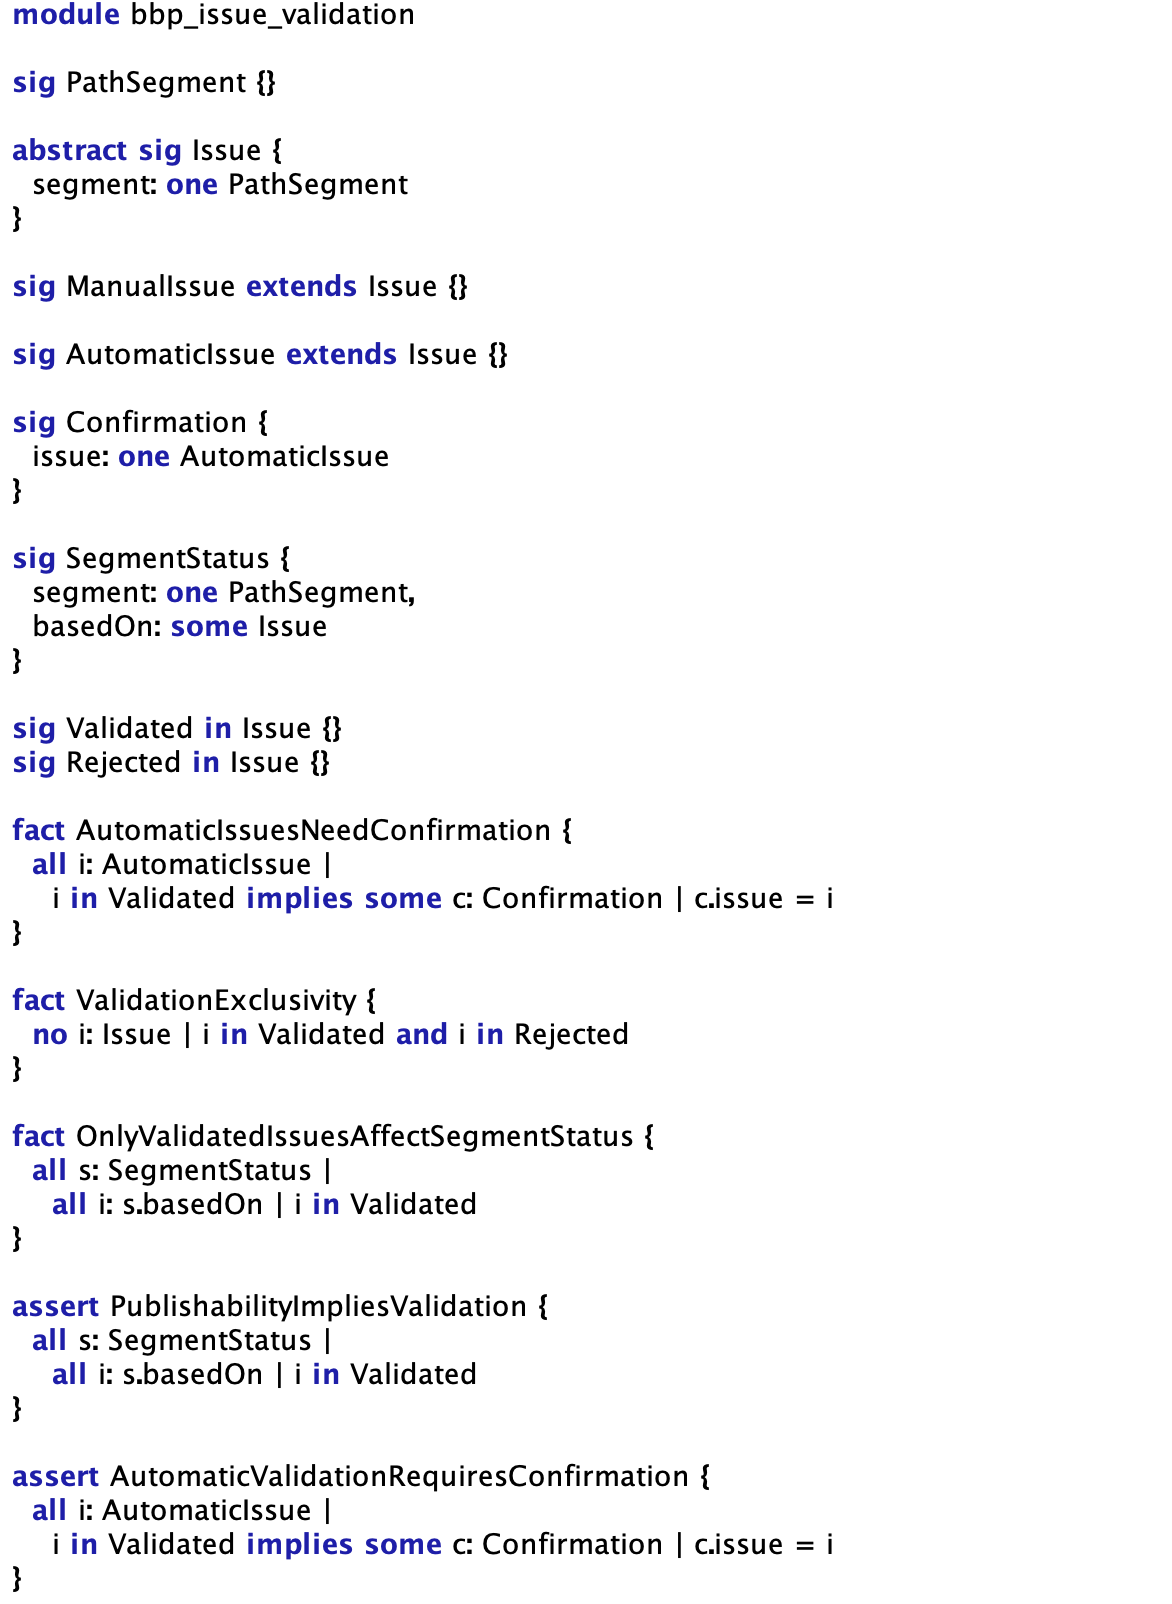
\includegraphics[width=\linewidth]{RASD/Figures/Full code 1.png}
    \caption{Alloy Code Part 1}
\end{figure}
\begin{figure}[H]
    \centering
    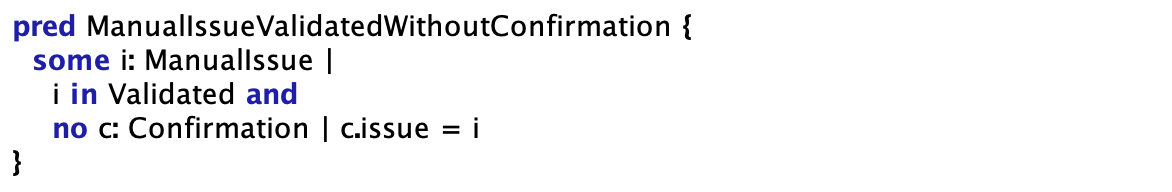
\includegraphics[width=\linewidth]{RASD/Figures/full code 2.png}
    \caption{Alloy Code Part 2}
\end{figure}
\begin{figure}[H]
    \centering
    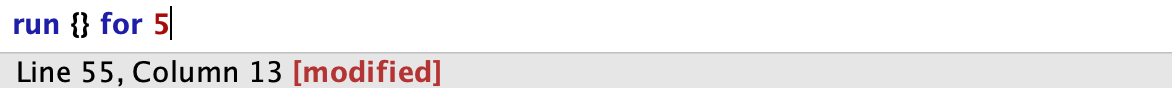
\includegraphics[width=\linewidth]{RASD/Figures/run code.png}
    \caption{Alloy Code Part 3}
\end{figure}
\begin{figure}[H]
    \centering
    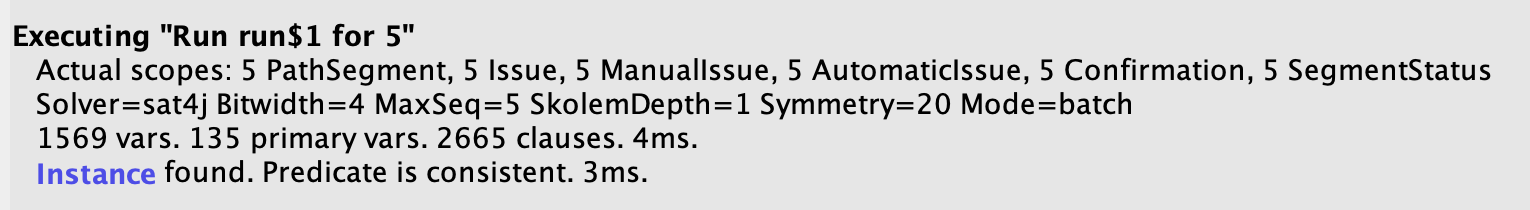
\includegraphics[width=\linewidth]{RASD/Figures/run output.png}
    \caption{Execution of the code}
\end{figure}

The Alloy model describes a simplified understanding of the BBP domain based on the issue lifecycle and their contribution to the publishable information for bike path segments. This model also assigns a collection of core elements based on the identified concepts from the specified domain. They also have exactly one path segment identified and issues classified based on their type and origins. They also have confirmations to indicate the endorsement of the identified issues by the users. They have a description and analysis of the rules governing the validation and publishability based on a collection of constraints. These constraints also indicate that the automatically identified issues can only achieve validation when there is at least one confirmation. They also indicate that the issues reported by users are assumed to have been validated by default. They also restrict issues rejected or failing validation from building the publishable information. They have abstract descriptions of the publishable information for the path segments based on the segment statuses derived solely from the validated issues. They restrict the possibility of invalidated or rejected issues to affect the information provided to the users based on their choices. This Alloy model determines the formal verification to notice whether the specified constraints on the validation and publishability of issues have logical soundness based on the selected scope without any deviation.\\

\begin{figure}[H]
    \centering
    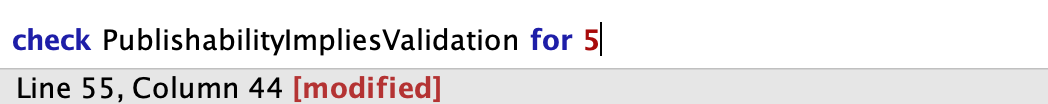
\includegraphics[width=\linewidth]{RASD/Figures/check publish code.png}
    \caption{Assertion and Check code part 1}
\end{figure}

\begin{figure}[H]
    \centering
    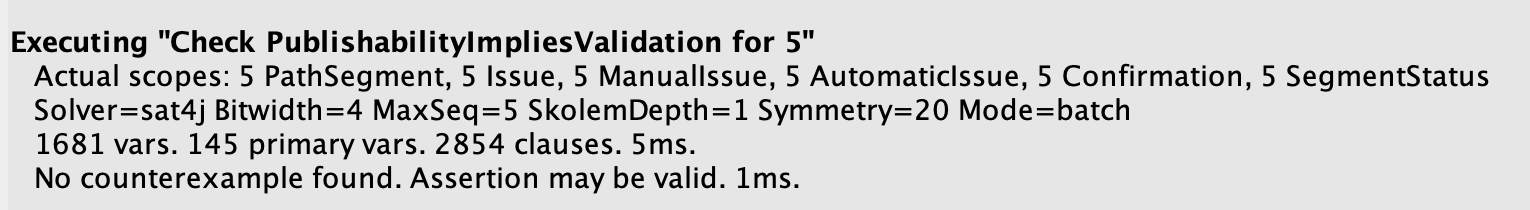
\includegraphics[width=\linewidth]{RASD/Figures/check publish output.png}
    \caption{Assertion and Check output part 1}
\end{figure}

\begin{figure}[H]
    \centering
    
\includegraphics[width=\linewidth]{RASD/Figures/check auto validation code.png}
    \caption{Assertion and Check code part 2}
\end{figure}

\begin{figure}[H]
    \centering
    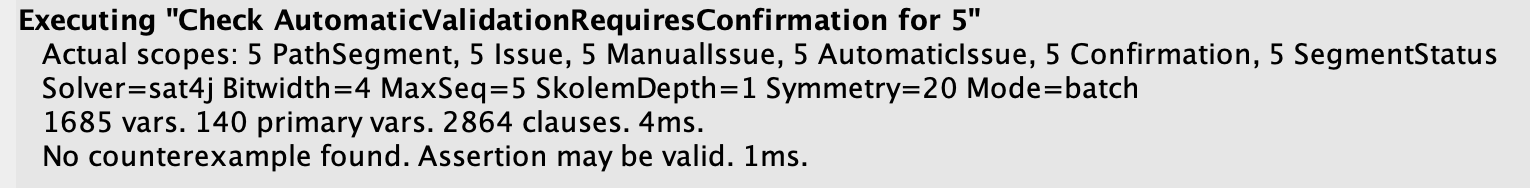
\includegraphics[width=\linewidth]{RASD/Figures/check auto validation output.png}
    \caption{Assertion and Check output part 2}
\end{figure}

To validate the correctness of the modeled constraints, we checked key properties through Alloy assertions. All checks were executed with a bounded scope of 5 instances for each signature. Alloy did not find counterexamples for the considered assertions, indicating that the modeled constraints enforce the intended requirements within the analyzed scope. Publishability implies validation. We verified that every issue contributing to publishable information (i.e., used by a segment status) must be validated. The check returned no counterexample found within the chosen scope. Automatic validation requires confirmation. We verified that an automatically detected issue cannot be validated unless at least one confirmation exists for that issue. The check returned no counterexample found within the chosen scope.

\begin{figure}[H]
    \centering
    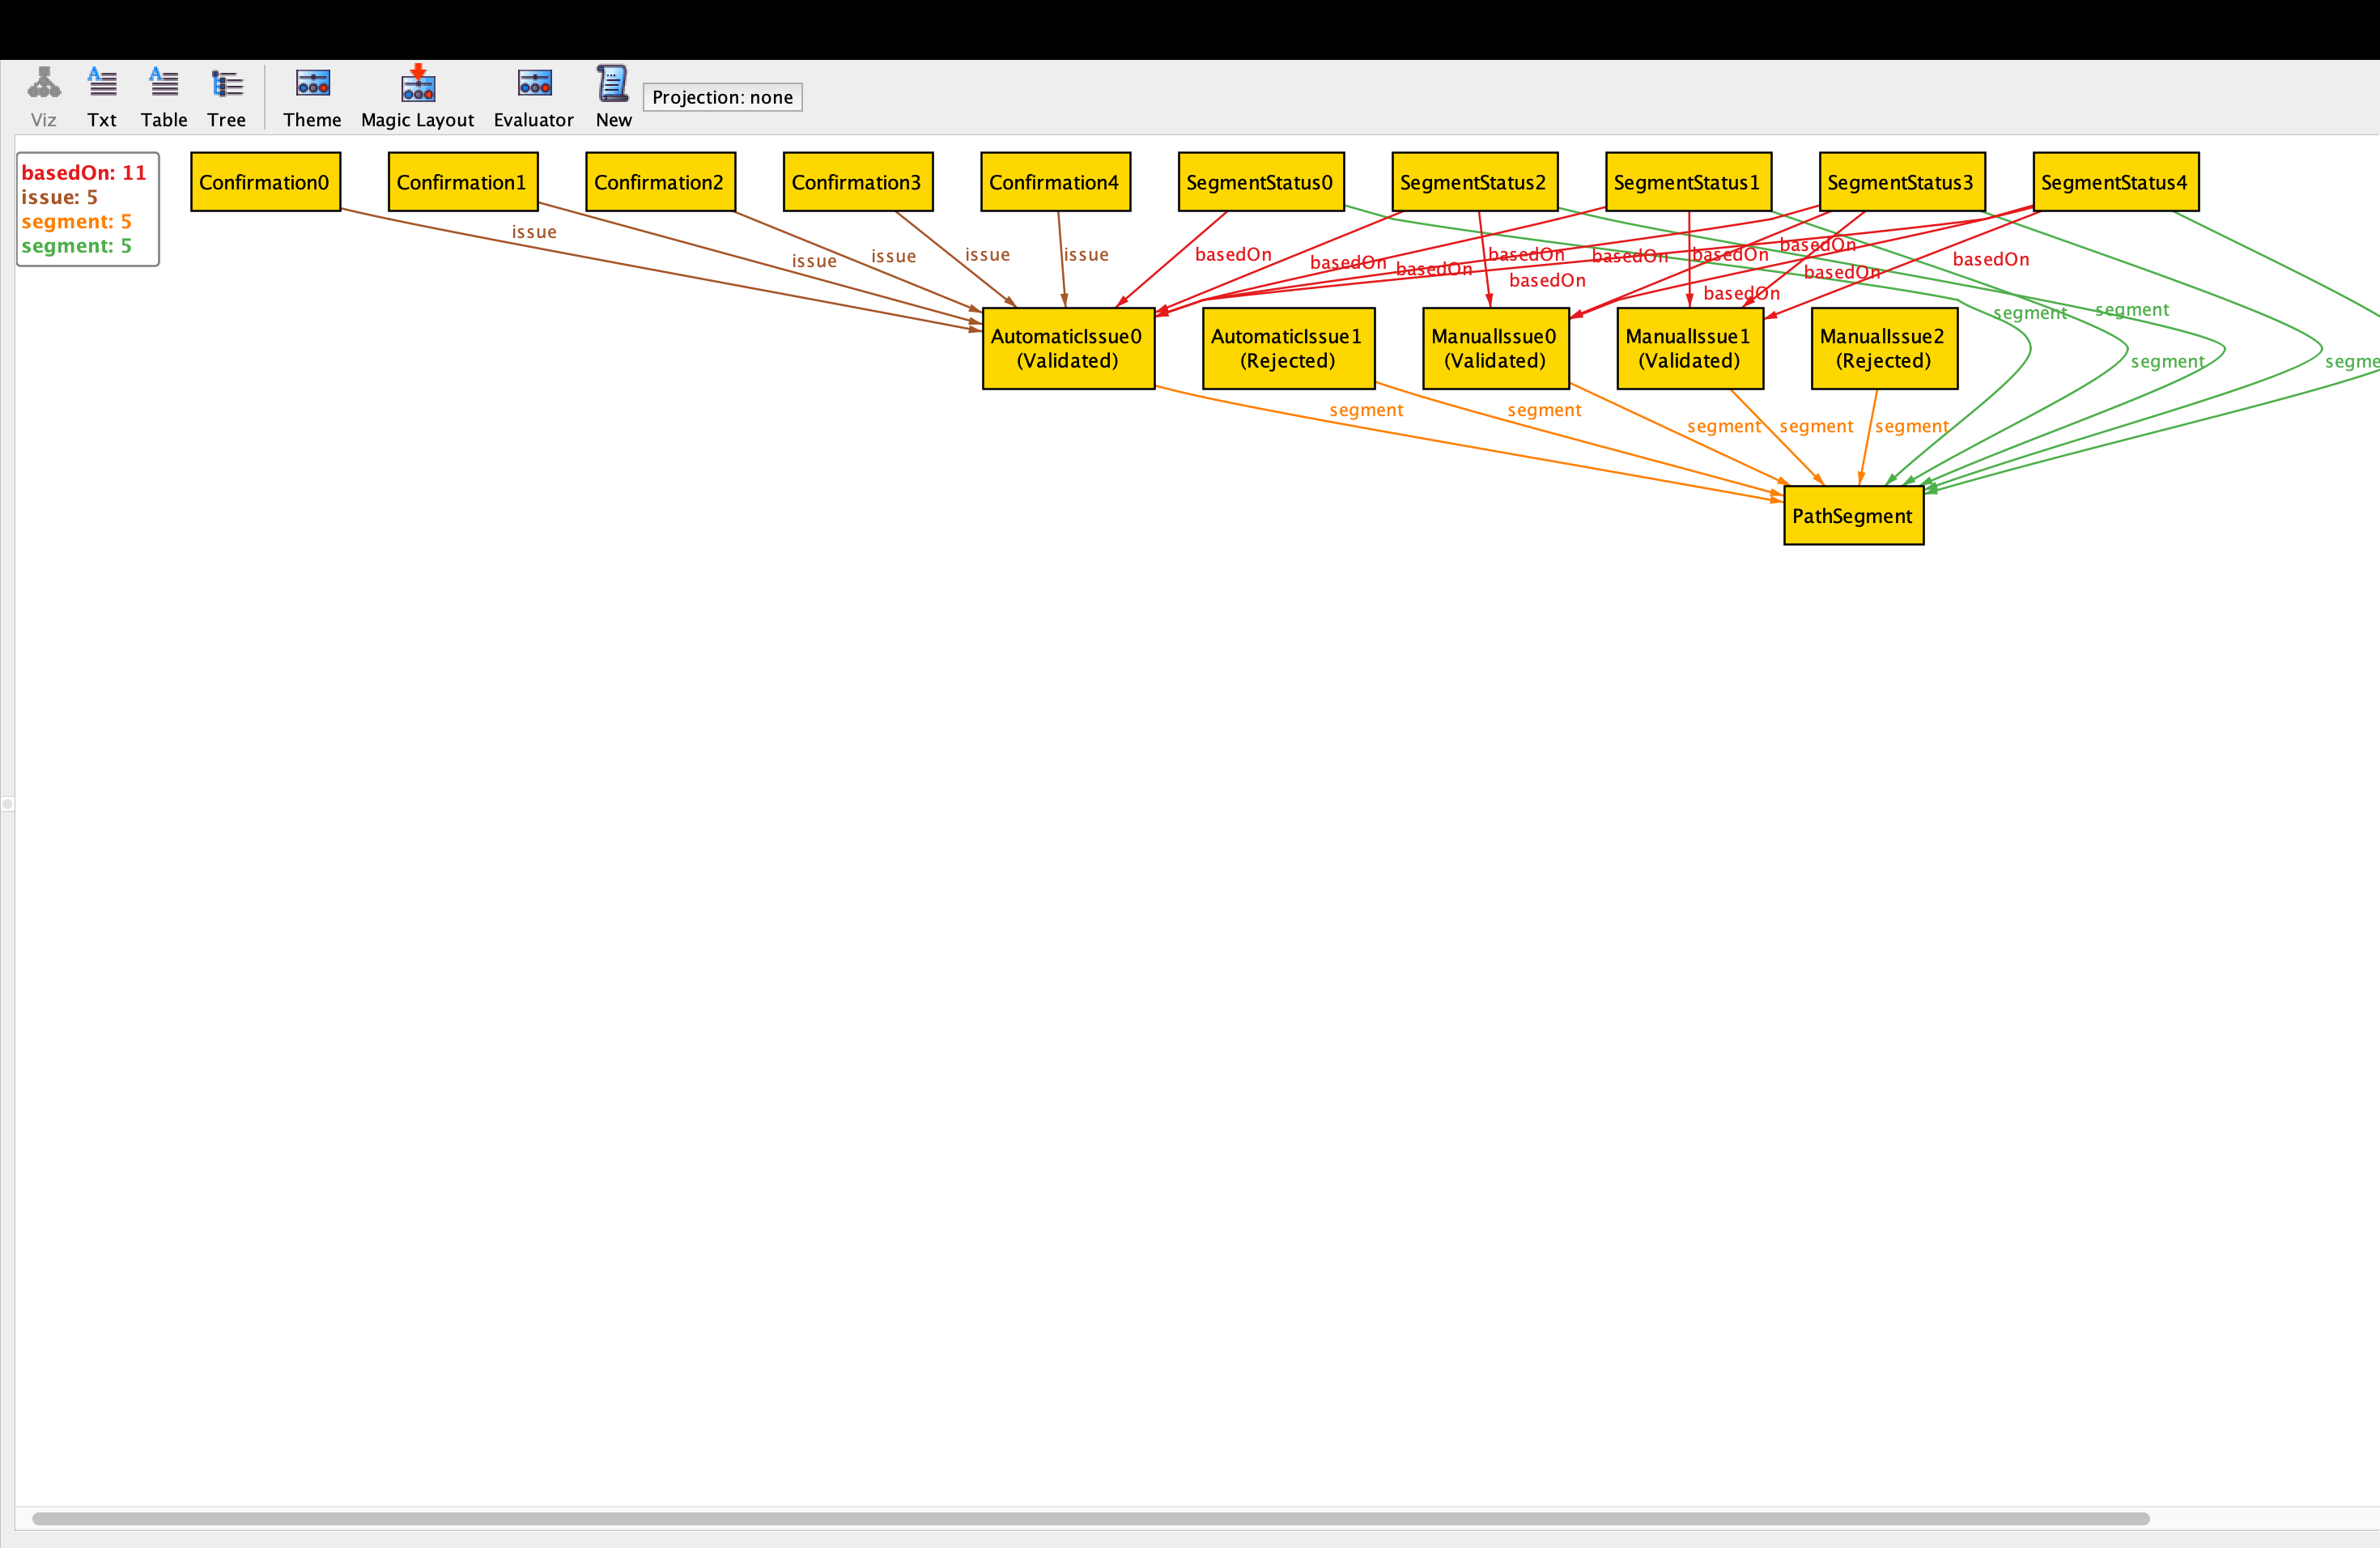
\includegraphics[width=\linewidth]{RASD/Figures/world 1.png}
    \caption{World 1 – Valid configuration of issues and segment statuses}
\end{figure}

This figure 25 illustrates a valid configuration of the Alloy model created by executing the model with no extra constraints. It includes both manually submitted and automatically identified issues. Automatically identified issues are checked only when they are tied with confirmations, whereas manually submitted issues can be checked directly. The segment statuses depend only on validated issues, which reinforces the belief that unvalidated or disqualified issues do not affect publishable paths.

\begin{figure}[H]
    \centering
    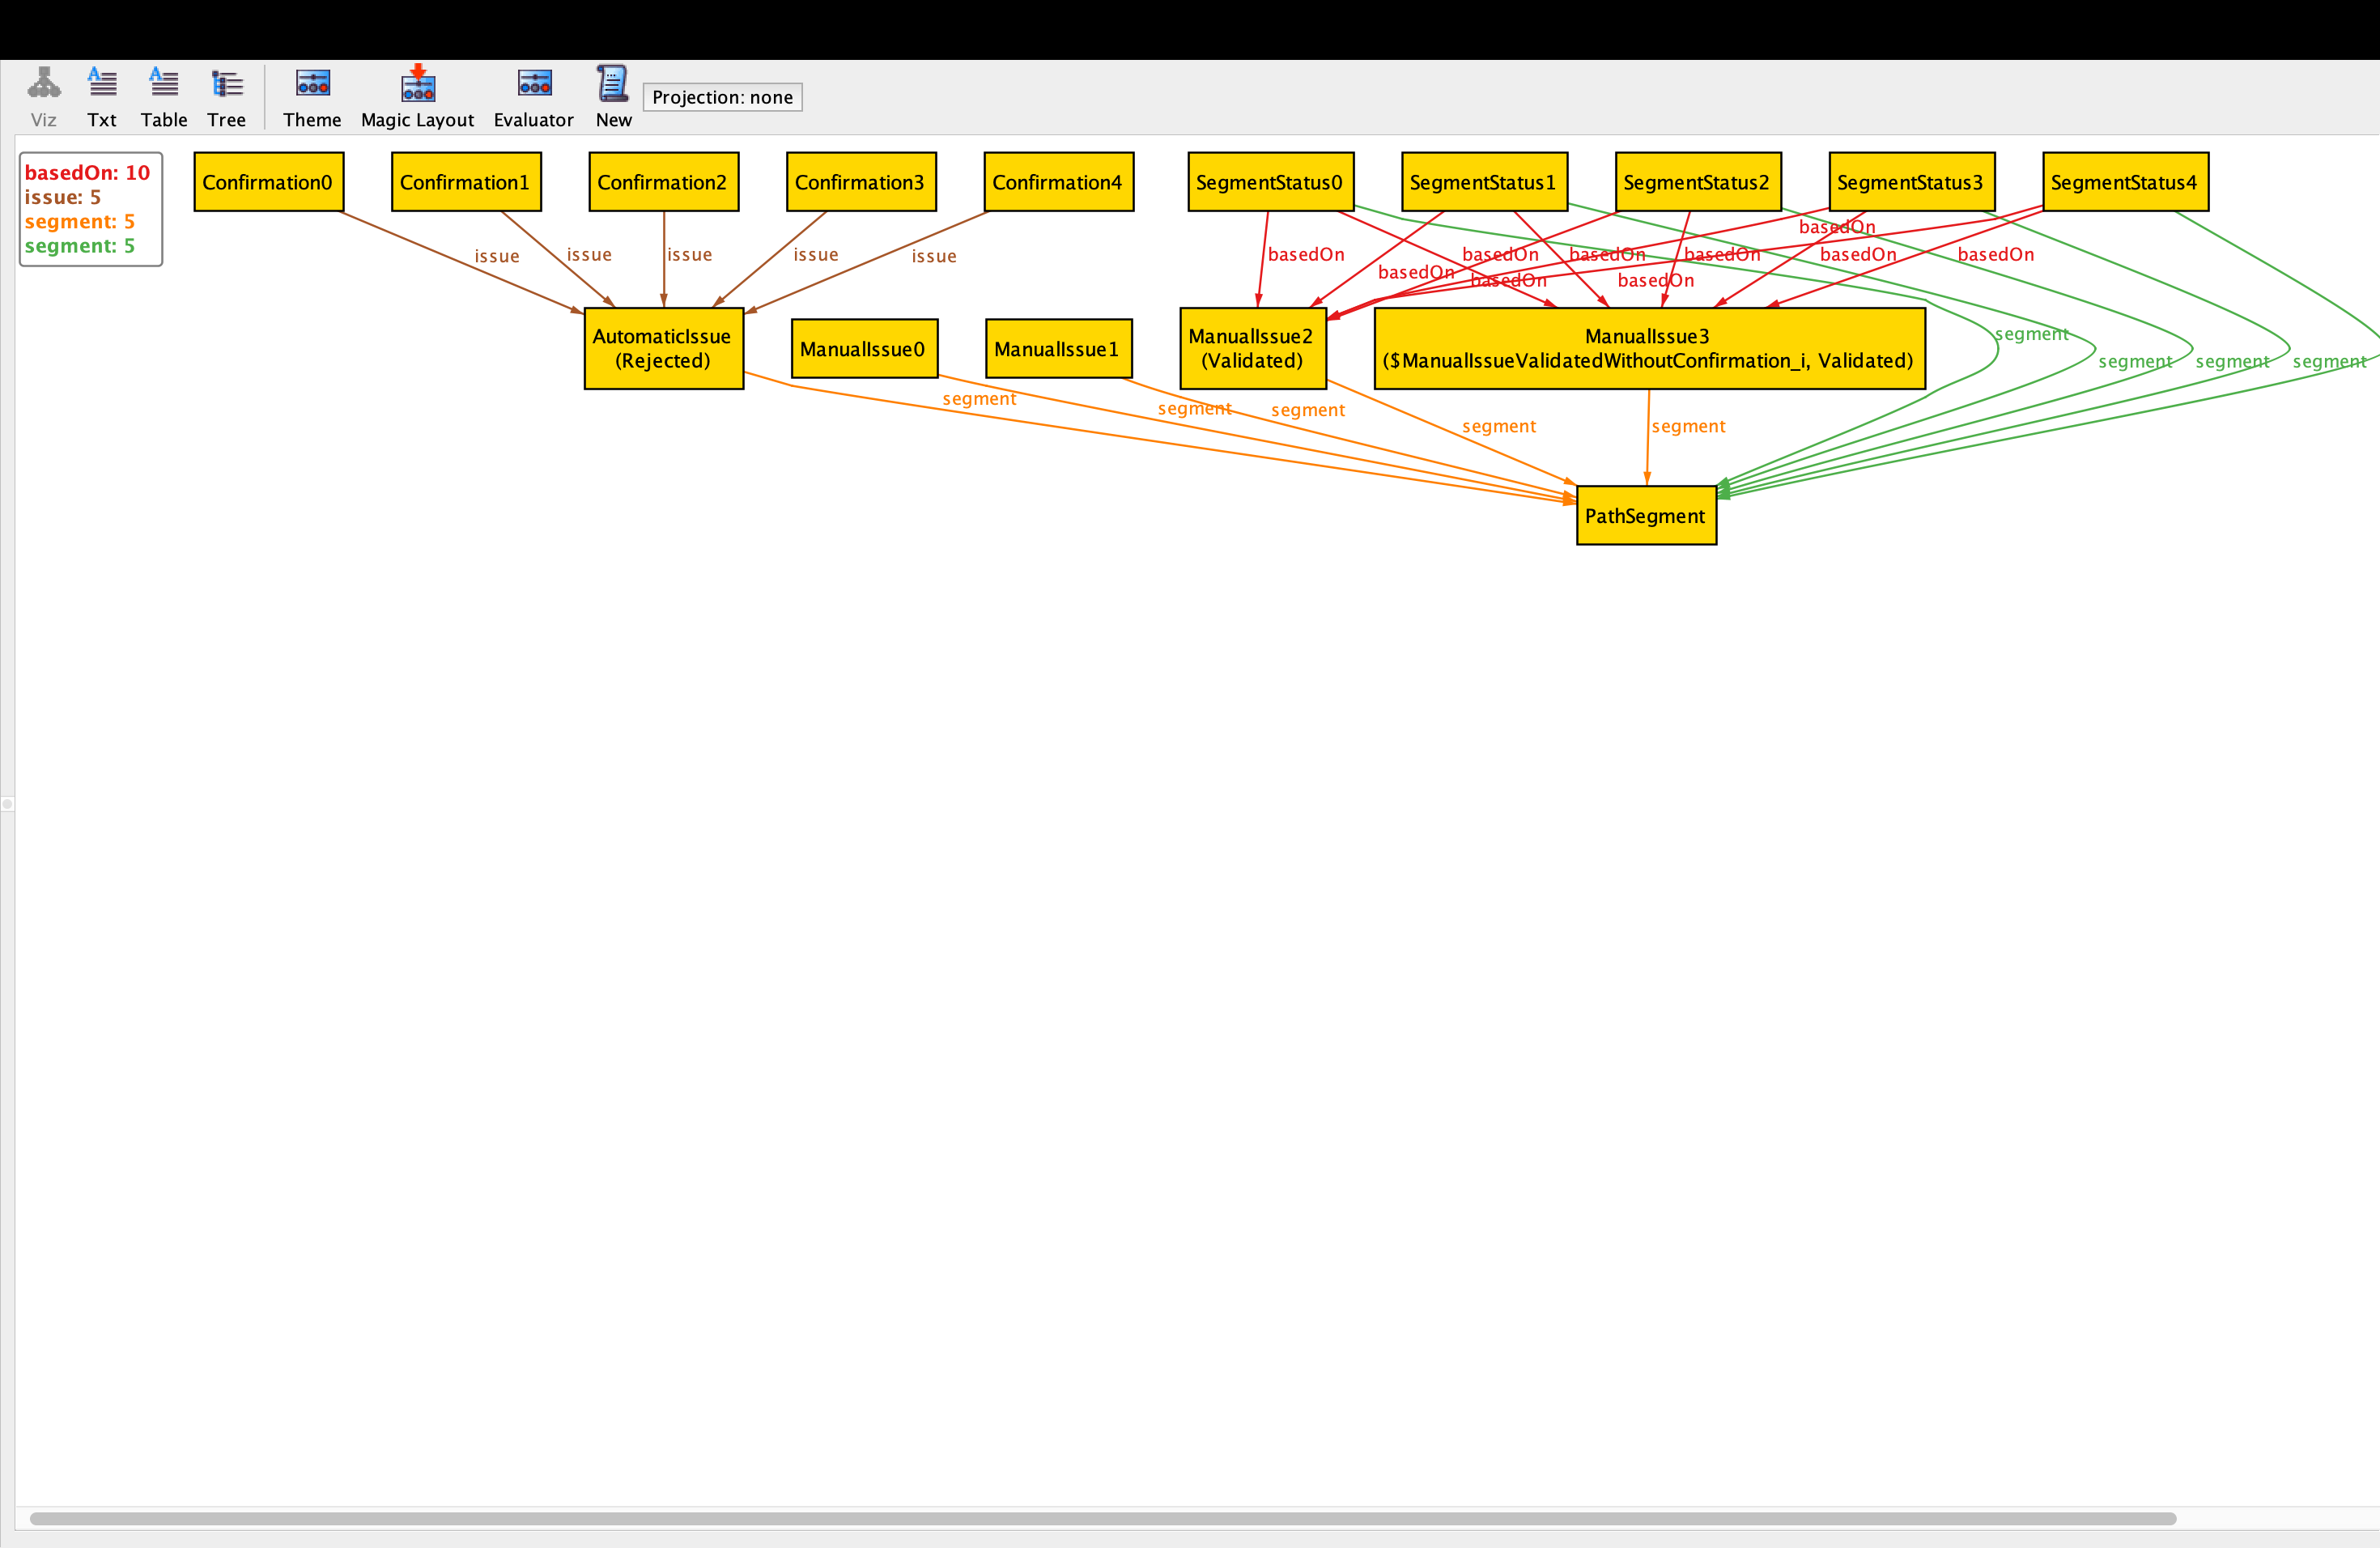
\includegraphics[width=\linewidth]{RASD/Figures/world 2.png}
    \caption{World 2 — Manual issue validated without confirmation}
\end{figure}

This figure 26 shows an instance generated by the predicate ManualIssueValidatedWithoutConfirmation. The instance contains a manually reported issue that is validated despite the absence of any confirmation. This execution demonstrates that the model correctly allows manual issues to be validated without confirmations, ensuring that validation rules are not over-constrained.

This formal verification confirms the logical correctness of the constraints regarding the validation of issues and publishability within the BBP system. Specifically, it checks that unparsed issues cannot be validated or affect publishable path information unless they are supported by user confirmations, and that only validated issues are reflected in segment statuses. These example executions also demonstrate that the model does not unduly constrain the system because manually entered issues can be validated without the need for confirmations. This verification largely confirms Goals G2, G3, and G6, as well as Use Case UC4.
